\documentclass[11pt,a4paper]{article}
% Packages
\usepackage{amsfonts}
\usepackage{amsmath}
\usepackage{amssymb}
\usepackage[hidelinks]{hyperref}
\usepackage{cleveref}
\usepackage{graphicx}
\usepackage[round]{natbib}
\usepackage{float,soul}
\usepackage{tikz}
\usepackage{caption}
\usepackage{tabularx}
\usepackage{xr}  % external document -- for supplements

\captionsetup[figure]{labelfont=bf,font=footnotesize}
\captionsetup[table]{labelfont=bf,font=footnotesize}

% Figure placement
\makeatletter
\def\fps@figure{tb}
\makeatother

% Newcommands
\DeclareMathSymbol{\shortminus}{\mathbin}{AMSa}{"39}  % useful for suffixes
\newcommand{\Ex}{\mathbb{E}}
\newcommand{\Var}{\mathrm{Var}}
\newcommand{\HW}{\mathrm{HW}}
\newcommand{\Bin}{\text{Binomial}}
\newcommand{\Uniform}{\text{Uniform}}
%\newcommand{\Normal}{\text{Normal}}
\newcommand{\Normal}{\mathcal{N}}
\newcommand{\Beta}{\text{Beta}}
\newcommand{\Exp}{\text{Exponential}}
\newcommand{\Gam}{\text{Gamma}}
\newcommand{\Bfun}{\mathrm{B}}
\newcommand{\eps}{\epsilon}
\newcommand{\logit}{\mathop{\mathrm{logit}}}
\newcommand{\Vx}{\mathcal{V}}



\usepackage{geometry}
\usepackage{authblk}
\externaldocument[m-]{main}
\renewcommand{\thefigure}{S\arabic{figure}}
\renewcommand{\thesection}{S\arabic{section}}
\renewcommand{\thealgorithm}{S\arabic{algorithm}}

\begin{document}
\title{Supplement: Autopolyploid establishment through polygenic adaptation}
\author{Arthur Zwaenepoel}
\date{\vspace{-5ex}}
\maketitle
\tableofcontents

\section{Supplementary Figures}

\begin{figure}[H]
\centering
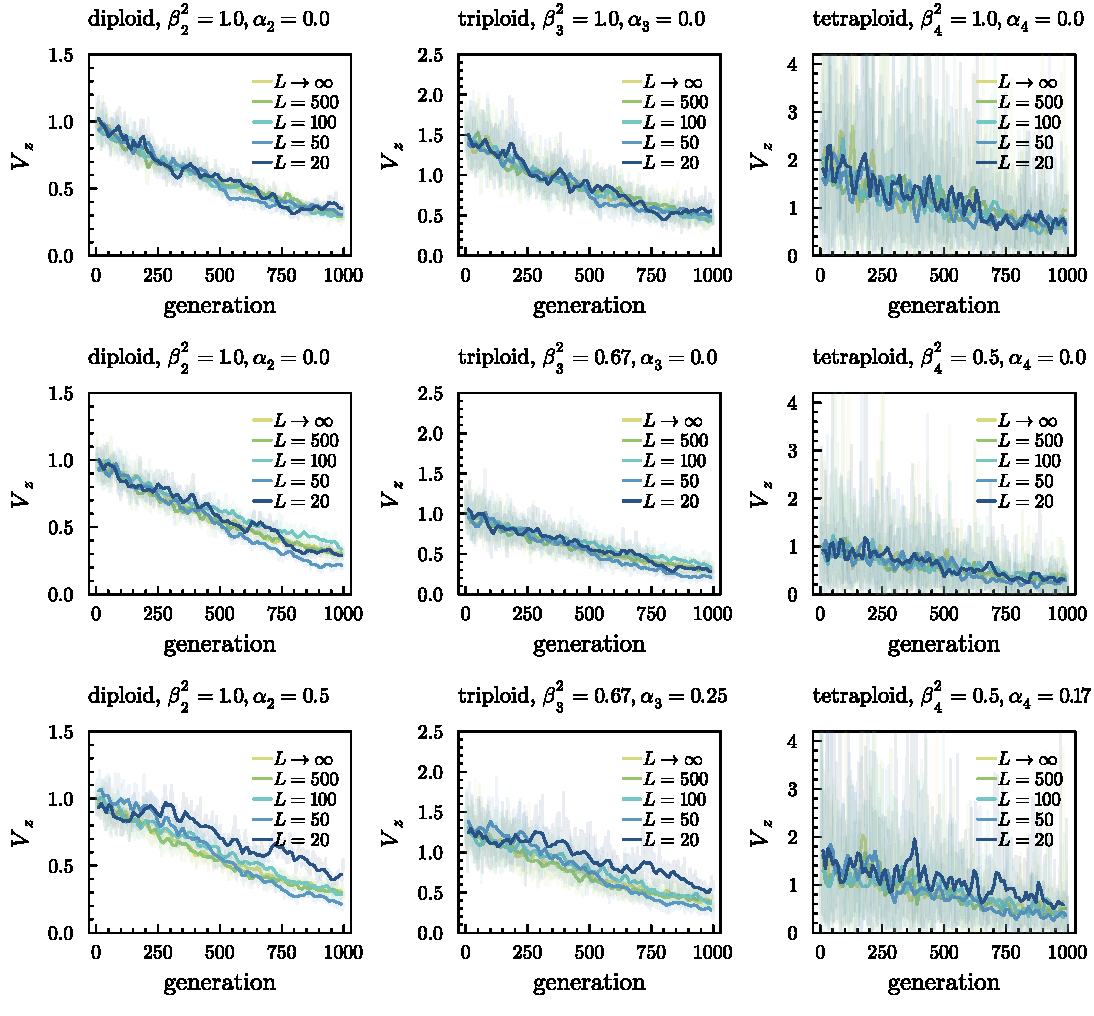
\includegraphics[width=\textwidth]{/home/arthur_z/vimwiki/build/img/2023-10-23/mixedploidy-Vz.pdf}
\caption{Comparison of the mixed-ploidy infinitesimal model with the
\(L\)-locus model, for \(L=500,100,50\) and \(20\). The decline in the
genetic variance \(V_z\) within each cytotype due to drift is shown. The
transparent lines show the complete simulation, whereas the solid line
shows the same data but smoothed in overlapping windows of 20
generations. We assume \(N=500, u=v=0.08\) and no selection. In the top
row where \(\beta_k^2=1, \alpha_k=0\), the equilibrium variance in the
absence of inbreeding in triploids is 2/3 that of diploids, and in
tetraploids it is twice that in diploids. In the middle row,
\(\beta_3^2=2/3\) and \(\beta_4^2=1/2\), so that the equilibrium
variance in the absence of inbreeding is equal across cytotypes. In the
bottom row, \(\alpha_2= \alpha_3 =1/2\) and \(\alpha_4=1/6\), causing an
immediate increase in the genetic variance in higher cytotypes, but also
accelerated inbreeding. \label{fig:vz}}
\end{figure}

\begin{figure}[H]
\centering
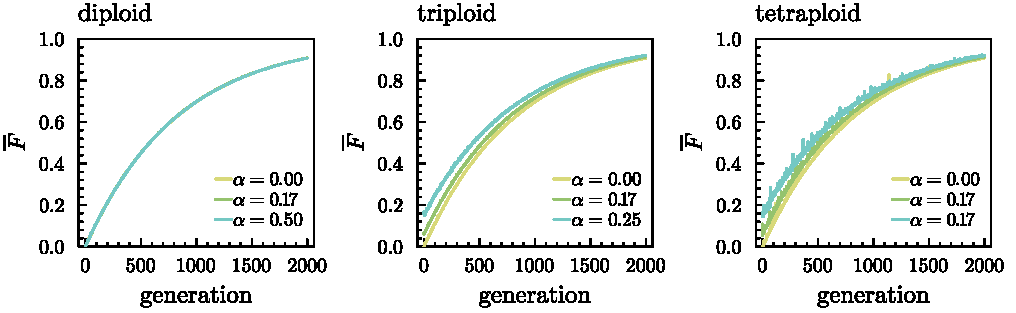
\includegraphics[width=\linewidth]{/home/arthur_z/vimwiki/build/img/2023-10-23/mixedploidy-F.pdf}
\caption{Average inbreeding coefficient \(\bar{F}\) in each cytotype in
a mixed-ploidy population for different values of \(\alpha\) (we assume
\(\alpha_k=\alpha\), where \(\alpha_k\) is the probability that a
diploid gamete produced by a \(k\)-ploid cytotype contains two copies of
the same parental gene at a random locus). We assume \(N=500, u=v=0.08\)
and no selection.}\label{fig:f1}
\end{figure}

\clearpage

\section{Supplementary Information}

\subsection{Inbreeding in autotetraploids \label{sec:tetinbred}}

In polyploids, the inbreeding coefficient $F_i$ does not suffice to describe
the state of homozygosity in individual $i$.
In tetraploids, for instance, we have five distinct homozygosity states, which
we can symbolically represent as $abcd, aabc, aabb, aaab$ and $aaaa$ (in
general, the number of homozygosity states grows according to the partition
function $(1,2,3,5,7,11,15,22,\dots)$).
Representing the probability of being in these five increasingly homozygous
states as $\delta_1, \dots, \delta_5$, we find that the gametic segregation
variance is reduced by a factor
  $$\phi = \delta_1 + \left(1 - \frac1 6\right) \delta_2 + \left(1 - \frac1
        3\right)\delta_3 + \left(1 - \frac1 2\right) \delta_4$$
which is precisely $1-F_i$, as in diploids (see also \cite{moody1993}).
This shows that we do not need to track the array of homozygosity coefficients
in order to compute the segregation variance in a tetraploid family, but only
require the inbreeding coefficients of the parents.
This is a consequence of the fact that, in tetraploids, gametes are diploid.
For higher ploidy levels, one would need to track higher order identity
coefficients.

Denoting the parents of individual $i$ by $k$ and $l$, the recursion for the
inbreeding coefficients in an autotetraploid population is
\begin{align}
    F_i &= \frac1 6 (F_k^\ast + F_l^\ast + 4\Phi_{kl}) \label{eq:rectet}
\end{align}
where $F_k^\ast = \alpha_4 + (1-\alpha_4)F_k$.
The recursion follows from considering three cases:
either (1) the two genes sampled in individual $i$ both came from the gamete
contributed by parent $k$, which happens with probability $1/6$, in which case
they are IBD with probability $F_k^\ast$; or (2) as in (1) but from parent $l$; or
(3) with probability $2/3$ the two genes came from different gametes, in which
case they are IBD with probability $\Phi_{kl}$ (the coancestry coefficient for
individuals $k$ and $l$).

\subsection{Mixed-ploidy infinitesimal model}

\subsubsection{Discrete locus model and variance scaling \label{sec:scaling}}

Consider an $L$-locus additive model, with two alleles (0 and 1) at each locus.
For a $k$-ploid individual, let $X_{i,j}$ be the allele at homolog $j$ of locus
$i$.
We assume the trait value is determined by
\begin{equation}
  z = \sum_{i=1}^L\sum_{j=1}^k a_{i,k} X_{i,j}
\end{equation}
Where $a_{i,k}$ is the allelic effect of the 1 allele at locus $i$ in
$k$-ploids.
The genetic variance at HWLE in $k$-ploids ($\tilde{V}_{z,k}$) will then be
\begin{equation}
  \tilde{V}_{z,k} = k\sum_{i=1} a_{i,k}^2 p_iq_i = kV_{x,k}
\end{equation}
where we refer to $V_{x,k}$ as the variance associated with a haploid genome in
$k$-ploids at HWLE.
Note that we also have $\tilde{V}_{z,2} = 2V_{x,k} = 2V$, where $V$ is the
segregation variance in the diploid population.

We now assume $a_{i,k} = \beta_k a_{i,2}$, i.e. allelic effects in $k$-ploids
are as in diploids, but scaled by a factor $\beta_k$.
This implies that
\begin{equation}
  \frac{\tilde{V}_{z,k}}{\tilde{V}_{z,2}} 
  = \frac{kV_{x,k}}{2V_{x,2}} = \frac{k}{2} \beta_{k}^2
\end{equation}
and hence also that $V_{x,k} = \beta_k^2 V_{x,2} = \beta_k^2 V$.
These relations will also hold in the infinitesimal limit.
Below, we derive the segregation variance expressions for the different meiotic
processes in the mixed-ploidy models in terms of the $V_{x,k}$.
Using the relationships outlined here, we will then be able to express all the
required variances in terms of $V$.

Note that under the above assumptions, not only the variance is rescaled, but
also the expected value of offspring within a family.
Specifically, for a $k$-ploid offspring of parental pair $i$ and $j$, where the
gamete coming from $i$ is $g_i$-ploid and the other gamete $g_j$-ploid, we have
\begin{equation}
  \Ex[Z_{ij}] = \beta_k \left(\frac{g_i}{c_i}\frac{z_i}{\beta_{c_i}} + 
    \frac{g_j}{c_j}\frac{z_j}{\beta_{c_j}}\right)
\end{equation}
where $c_i$ is the ploidy level of individual $i$.
Here we rescale the parental trait values to the diploid scale by dividing by
$\beta_{c_i}$, sum the expected rescaled gametic values, and rescale to the
offspring ploidy level.

\subsubsection{Segregation variance \label{sec:segvar}}

\subsection{Deterministic mixed-ploidy model \label{sec:det}}

Let $g_k$ be the frequency of $k$-ploid gametes in the gamete pool, and let us
consider only haploid and diploid gametes, so that $g_2 = 1-g_1$.
Diploids produce unreduced gametes with probability $u$ and reduced ones with
probability $1-u$, triploids produce haploid and triploid gametes both with
probability $v$, and tetraploids produce reduced diploid gametes with
probability $(1-u)$ (we assume they produce, just like diploids, a proportion
$u$ of unreduced gametes, but these are assumed not to lead to viable offspring
and are ignored).
We get after one generation of random mating
  $$g_1' = \frac{(1-u)g_1^2 + 2vg_1g_2}{g_1^2 + 4vg_1g_2 + (1-u)g_2^2}.$$
We see that $g_1=0$ is always an equilibrium (no haploid gametes, tetraploids
take over).
Two more fixed points are obtained at
  \begin{equation}
  \tilde{g_1}, \tilde{g_1}' =
    \frac{3 - 3u - 6v \pm \sqrt{(u + 2v - 1)(5u + 2v - 1)}}
         {2(2 - u - 4v)} \label{eq:gameteq}
  \end{equation}
Of which the larger one, when it exists, corresponds to a stable equilibrium,
and the smaller one to an unstable equilibrium.
As there are no viability differences, the equilibrium cytotype frequencies can
be readily obtained from these through the relations 
\begin{align}
\pi_2 = \tilde{g_1}^2 & & \pi_3 = 2\tilde{g_1}\tilde{g_2} & & 
    \pi_4 = \tilde{g_2}^2
\label{eq:cyteq}
\end{align}
Assuming $v=O(u)$, we have to second order in $u$
\begin{align}
 \pi_2 &= 1 - 2u - 4uv - u^2 + O(u^3)  \nonumber \\
 \pi_3 &= 2u + 4uv + O(u^3) \nonumber \\
 \pi_4 &= u^2 + O(u^3) 
\end{align}
At the critical point where the stable equilibrium disappears, we have that
$\Delta g_1 = \frac{d\Delta g_1}{d g_1} = 0$ (\cref{fig:g1diff}, middle).
We find that, in the region of parameter space that is biologically relevant
(roughly $u < 0.1, v < 0.1$, say), the critical unreduced gamete formation rate
$u_c$ beyond which tetraploids take over can be expressed as a linear function
of triploid fertility ($2v$):
  $$u_c = \frac{1}{5}(1-2v)$$
(\cref{fig:g1diff}, right).
This shows that, for plausible parameter values, we can safely assume that an
initially diploid population will evolve to a mixed-ploidy equilibrium.
A similar model was first analyzed in \cite{felber1997}.

\begin{figure}
\centering
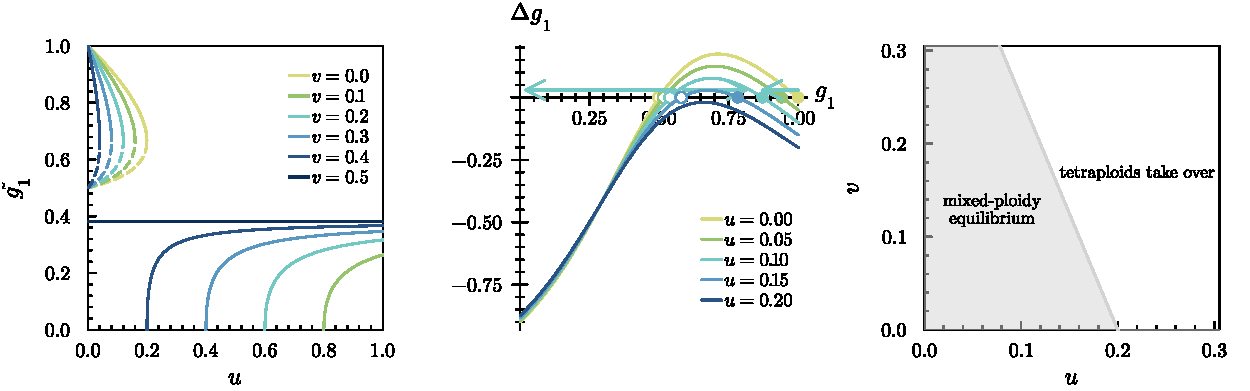
\includegraphics[width=\linewidth]{/home/arthur_z/vimwiki/build/img/2023-10-13/g1diff.pdf}
\caption{
Deterministic mixed-ploidy equilibrium. The left plot shows the stable (solid
lines) and unstable (dashed lines) equilibria for the proportion of haploid
gametes in the gamete pool $g_1$ as a function of $u$ for different values of
$v$. The middle plot shows the relationship between $\Delta g_1 = g_1' - g_1$
and $g_1$. The zeros of this graph are the fixed points of the dynamical system
and are indicated by the hollow (unstable equilibrium) and solid (stable
equilibrium) dots. The rightmost plot shows the region of parameter space where
a stable mixed-ploidy equilibrium exist.
\label{fig:g1diff}}
\end{figure}

\subsection{Stochastic mixed-ploidy model \label{sec:mchain}}

For finite $N$, the basic mixed-ploidy model defines a Markov chain on the
state space $[0..N] \times [0..N]$.
\begin{align}
  p_{ij,kl} = \Pr\{N_2(t+1)=k,& N_3(t+1)=l | N_2(t)=i, N_3(t)=j\} \nonumber \\
    &= \frac{N!}{k!l!(N-k-l)!} p_2^k p_3^l (1-p_2-p_3)^{N-k-l}
\end{align}
where 
\begin{align}
  p_2 &= \left(\frac{i(1-u) + jv}{N(1-u) + (i+j)u + j(2v-1)}\right)^2 \\
  p_3 &= \left(\frac{2(i(1-u) + jv)(N(1-u) + i(2u - 1) + j(u + v - 1))}
    {N(1-u) + (i+j)u + j(2v-1)}\right)^2 
\end{align}
Associating a unique index with each pair $(i,j)$ with $0 \le i,j \le N$, we
can define a transition probability matrix $P$ of dimensions $(N+1)^2 \times
(N+1)^2$ for this Markov chain.

For nonzero $u$ and $v$, the only absorbing state is the one where $N_2 = N_3 =
0$, i.e. the tetraploid cytotype fixes.
All other states are transient, and hence tetraploid fixation occurs with
probability one.
The expected time until fixation may however be extremely long.
Using standard theory for absorbing Markov chains, we can numerically compute
the expected time until fixation $\Ex[T_{\text{fix}}]$ from the transition
probability matrix.
Calculations for the case where $u=v=0.05$ (which are large parameter values
conducive for tetraploid fixation) are shown in \cref{tbl:mchain-ex}.  Clearly,
tetraploid establishment by drift alone requires very small population sizes to
occur at an appreciable rate.
A similar model without triploids has been analyzed by \cite{rausch2005}.

\begin{table}[t]
\caption{
Expected number of generations until fixation of the tetraploid cytotype for
different population sizes, assuming $u=v=0.05$ and an initially diploid
population. \label{tbl:mchain-ex}
}
\begin{tabularx}{\linewidth}{XXXXXX}
\cline{1-6}
$N$ & 10 & 20 & 30 & 40 & 50 \\
\cline{1-6}
$\Ex[T_{\text{fix}}]$ & $5.4 \times 10^3$ & $6.4 \times 10^5$ & 
    $7.9 \times 10^7$ & $9.8 \times 10^9$ & $1.2 \times 10^{12}$ 
\end{tabularx}
\end{table}

\subsection{Expected time to diploid ancestry \label{sec:ttdip}}

Consider a gene sampled from a tetraploid individual in a mixed-ploidy
population at equilibrium and not subjected to selection. Let \(T_4\)
denote the number of generations in the past until such a gene is found
in a diploid ancestor, and let \(T_3\) denote a similar random variable
for a randomly sampled gene from a triploid in the same population.
Assuming the different cytotypes are at their deterministic equilibrium
frequencies \(\pi_2, \pi_3\) and \(\pi_4\) (see sec.~\ref{sec:det},
eq.~\ref{eq:cyteq}), we have the recursive relations \begin{align}
  \Ex[T_4] &= \frac{1}{Z_2}\Big(\pi_2u + (1+\Ex[T_3])\pi_3 v +
    (1+\Ex[T_4])\pi_4(1-u)\Big) \nonumber \\
  \Ex[T_3] &= \frac{1}{3Z_1}\Big(\pi_2(1-u) + (1+\Ex[T_3])\pi_3 v\Big)
  \nonumber
    \\ &\qquad + \frac{2}{3Z_2}\Big(\pi_2 u + (1+\Ex[T_3])\pi_3 v +
      (1+\Ex[T_4])\pi_4(1-u)\Big) \label{eq:ttdip}
\end{align} where \begin{align*}
  Z_1 &= \pi_2(1-u) + \pi_3v \\
  Z_2 &= \pi_2u + \pi_3v + \pi_4(1-u)
\end{align*} (these expressions are straightforwardly modified when more
general \(u_{ij}\) are assumed, see e.g. sec.~\ref{sec:effsize},
eq.~\ref{eq:markovch}). The system in eq.~\ref{eq:ttdip} can be solved
to yield expressions for \(\Ex[T_4]\) and \(\Ex[T_3]\), which are
however rather unwieldy. Again assuming \(v=O(u)\), we obtain to first
order in \(u\) \begin{align*}
\Ex[T_4] &= 1 + u + 2v + O(u^2) \\
\Ex[T_3] &= 1 + \frac{2}{3}(u + 2v) + O(u^2) 
\end{align*} Numerical examples are shown in (fig.~\ref{fig:ttdip}).
Clearly, for plausible parameter values, \(\Ex[T]\) will be very close
to 1. For instance, for \(u=0.05\) and \(v=0.05\) (which are already
rather large values for these parameters), we would have
\(\Ex[T_3] \approx 1.13\) and \(\Ex[T_4] \approx 1.19\).


\begin{figure}
\centering
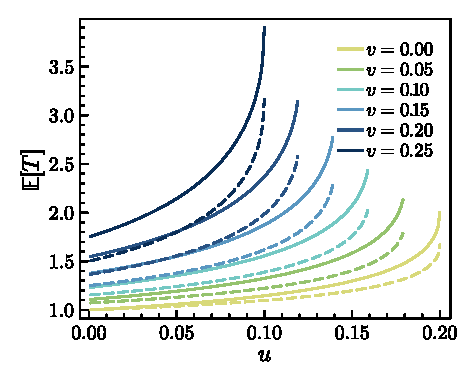
\includegraphics[width=0.5\textwidth]{/home/arthur_z/vimwiki/build/img/2023-10-22/timetodiploidancestord.pdf}
\caption{Expected time to diploid ancestry. The solid lines show
\(\Ex[T_4]\), i.e.~the expected time since being inherited from a
diploid ancestor for a random gene in a tetraploid individual at
equilibrium, for different values of \(v\) (half the triploid
fertility). The dashed lines show \(\Ex[T_3]\), i.e.~the same quantity
for a gene sampled from a triploid. Note that \(\Ex[T]\) blows up
whenever \(u\) and \(v\) exceed their critical value for tetraploid
establishment. \label{fig:ttdip}}
\end{figure}

\subsection{Effective population size of a mixed-ploidy deme \label{sec:effsize}}

\begin{figure}
\centering
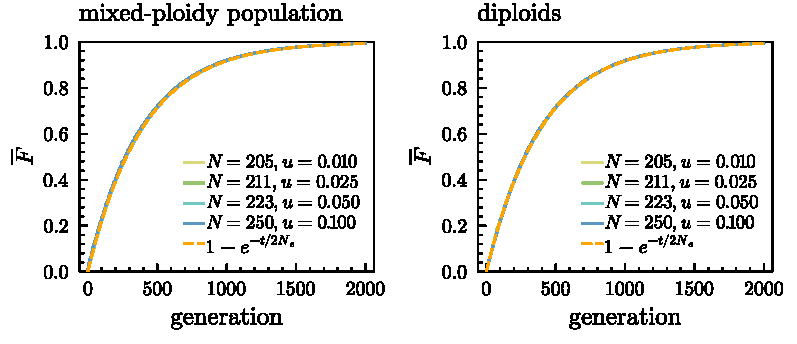
\includegraphics[width=\textwidth]{/home/arthur_z/vimwiki/build/img/2023-10-13/mixedploidy-F-Ne.pdf}
\caption{The evolution of \(\bar{F}\) in the mixed-ploidy population and
in the diploid subpopulation are shown for different values of \(u\) and
associated values of \(N\), keeping \(N_e = (1-2u)N\) constant at 200.
We assume \(u=v\). All lines coincide almost completely and are
indistinguishable from \(1-e^{-t/2N_e}\). Results are shown for
\(\alpha_k=1/6\). As \(\alpha_k\) decreases to 0, \(\bar{F}\) in the
mixed-ploidy population becomes completely indistinguishable from
\(\bar{F}\) in the diploid subpopulation.}\label{fig:fNe}
\end{figure}

We use the approach outlined in \citep{rousset2004} (pp.~153, 157) to
determine the effective size of a randomly mating mixed-ploidy
population. Denote by \(\nu_k(t)\) the probability that the ancestral
lineage of a given gene in the present is found in a individual of
ploidy level \(k\) \(t\) generations in the past, and let
\(\nu(t) = (\nu_2(t)\ \nu_3(t)\ \nu_4(t))\) be the corresponding row
vector. Assuming the population is at cytotype equilibrium
(eq.~\ref{eq:cyteq}), we have 
  \begin{align}
      \nu(t+1) &= \nu(t) P \nonumber \\
               &= \nu(t) \begin{pmatrix}
      \frac{u_{21}}{Z_1}\pi_2 & \frac{u_{31}}{Z_1}\pi_3 & 0 \\
      \left(\frac{u_{21}}{3Z_1} + \frac{2u_{22}}{3Z_2}\right)\pi_2 &
          \left(\frac{u{31}}{3Z_1} + \frac{2u_{32}}{3Z_2}\right)\pi_3 & 
          \frac{2u_{42}}{3Z_2}\pi_4 \\
      \frac{u_{22}}{Z_2}\pi_2 & \frac{u_{32}}{Z_2}\pi_3 & \frac{u_{42}}{Z_2}\pi_4
      \label{eq:markovch}
       \end{pmatrix}
  \end{align}
where we assume, as usual, that tetraploids do not
produce haploid gametes (\(u_{41} = 0\)), and where \begin{align*}
  Z_1 &= u_{21} \pi_2+ u_{31} \pi_3 \\
  Z_2 &= u_{22} \pi_2 + u_{32} \pi_3 + u_{42} \pi_4
\end{align*} At stationarity,
\(\lim_{t\rightarrow \infty} \nu(t) = \nu\), and we have
\(\nu = \nu P\). Hence, the probability that the ancestral lineage of a
given gene in the present is found in an individual of ploidy level
\(k\) in an indefinite past is given by \(\nu_k\), where \(\nu\) is the
left eigenvector of \(P\) associated with the unit eigenvalue. The
effective size of a mixed-ploidy population of size \(N\) can then be
obtained as \[N_e = N\left(\sum_k \frac{\nu_k^2}{\pi_k}\right)^{-1}\]
After plugging in \(\pi\) in accordance with eq.~\ref{eq:cyteq} and
solving the eigenvalue problem, this yields an unwieldy expression in
the \(u_{ij}\). For our usual parameterization where
\(u_{21} = u_{42} = 1-u, u_{22} = u\) and \(u_{31} = u_{32} = v\), and
\(v = O(u)\), we can find that
\[\begin{pmatrix}\nu_2 \\ \nu_3 \\ \nu_4\end{pmatrix} = \begin{pmatrix}
    1-2uv + O(u^3) \\ 2uv + O(u^3) \\ O(u^3)\end{pmatrix}\] and
\[\frac{N_e}{N} = 1 - 2u + O(u^2)\] which yields an excellent fit in
simulations for plausible parameter values (fig.~\ref{fig:fNe}). When
\(v=0\) and \(u < u_c\) (see sec.~\ref{sec:det}), \(N_e = \pi_2N\), as
in that case (i.e.~when triploids are infertile) there can be no gene
flow from tetraploids to diploids. Since we assume the cytotype
composition to be constant, and polyploids are continually formed from
diploids, no gene in a triploid or tetraploid will have any descendants
in the distant future in this case, so that the effective size is just
the diploid fraction of the population.

\bibliographystyle{abbrvnat}
\bibliography{/home/arthur_z/vimwiki/bib.bib}
\end{document}
